\documentclass[11pt,]{article}
\usepackage[]{mathpazo}
\usepackage{amssymb,amsmath}
\usepackage{ifxetex,ifluatex}
\usepackage{fixltx2e} % provides \textsubscript
\ifnum 0\ifxetex 1\fi\ifluatex 1\fi=0 % if pdftex
  \usepackage[T1]{fontenc}
  \usepackage[utf8]{inputenc}
\else % if luatex or xelatex
  \ifxetex
    \usepackage{mathspec}
  \else
    \usepackage{fontspec}
  \fi
  \defaultfontfeatures{Ligatures=TeX,Scale=MatchLowercase}
\fi
% use upquote if available, for straight quotes in verbatim environments
\IfFileExists{upquote.sty}{\usepackage{upquote}}{}
% use microtype if available
\IfFileExists{microtype.sty}{%
\usepackage{microtype}
\UseMicrotypeSet[protrusion]{basicmath} % disable protrusion for tt fonts
}{}
\usepackage[margin=1in]{geometry}
\usepackage{hyperref}
\hypersetup{unicode=true,
            pdftitle={Historical declines in snail body size at population and assemblage scales},
            pdfauthor={Robin Elahi},
            pdfborder={0 0 0},
            breaklinks=true}
\urlstyle{same}  % don't use monospace font for urls
\usepackage{longtable,booktabs}
\usepackage{graphicx,grffile}
\makeatletter
\def\maxwidth{\ifdim\Gin@nat@width>\linewidth\linewidth\else\Gin@nat@width\fi}
\def\maxheight{\ifdim\Gin@nat@height>\textheight\textheight\else\Gin@nat@height\fi}
\makeatother
% Scale images if necessary, so that they will not overflow the page
% margins by default, and it is still possible to overwrite the defaults
% using explicit options in \includegraphics[width, height, ...]{}
\setkeys{Gin}{width=\maxwidth,height=\maxheight,keepaspectratio}
\IfFileExists{parskip.sty}{%
\usepackage{parskip}
}{% else
\setlength{\parindent}{0pt}
\setlength{\parskip}{6pt plus 2pt minus 1pt}
}
\setlength{\emergencystretch}{3em}  % prevent overfull lines
\providecommand{\tightlist}{%
  \setlength{\itemsep}{0pt}\setlength{\parskip}{0pt}}
\setcounter{secnumdepth}{0}
% Redefines (sub)paragraphs to behave more like sections
\ifx\paragraph\undefined\else
\let\oldparagraph\paragraph
\renewcommand{\paragraph}[1]{\oldparagraph{#1}\mbox{}}
\fi
\ifx\subparagraph\undefined\else
\let\oldsubparagraph\subparagraph
\renewcommand{\subparagraph}[1]{\oldsubparagraph{#1}\mbox{}}
\fi

%%% Use protect on footnotes to avoid problems with footnotes in titles
\let\rmarkdownfootnote\footnote%
\def\footnote{\protect\rmarkdownfootnote}

%%% Change title format to be more compact
\usepackage{titling}

% Create subtitle command for use in maketitle
\newcommand{\subtitle}[1]{
  \posttitle{
    \begin{center}\large#1\end{center}
    }
}

\setlength{\droptitle}{-2em}
  \title{Historical declines in snail body size at population and assemblage
scales}
  \pretitle{\vspace{\droptitle}\centering\huge}
  \posttitle{\par}
  \author{Robin Elahi}
  \preauthor{\centering\large\emph}
  \postauthor{\par}
  \predate{\centering\large\emph}
  \postdate{\par}
  \date{2018-01-16}


\begin{document}
\maketitle

\subsection{Abstract}\label{abstract}

We explored historical changes in body size at the population and
assemblage scales using a suite of herbivorous snails on a rocky shore
in central California. At the population scale, we tested for changes in
the body size of three species (\emph{Chlorostoma funebralis},
\emph{Lottia digitalis}, \emph{Littorina keenae}) using size-frequency
data at two time points separated by six decades. Snails are now
smaller. At the assemblage scale, we tested whether maximum body size
predicted the abundance trends of 11 herbivorous snails over nine
decades on the same rocky shore. Smaller-bodied snails are now more
abundant, while larger-bodied snails are less abundant. We discuss these
observations in the context of potential mechanisms, including climate
change and recruitment variability, as well as the consequences of such
widespread shifts in body size.

\newpage

\subsection{Figures}\label{figures}

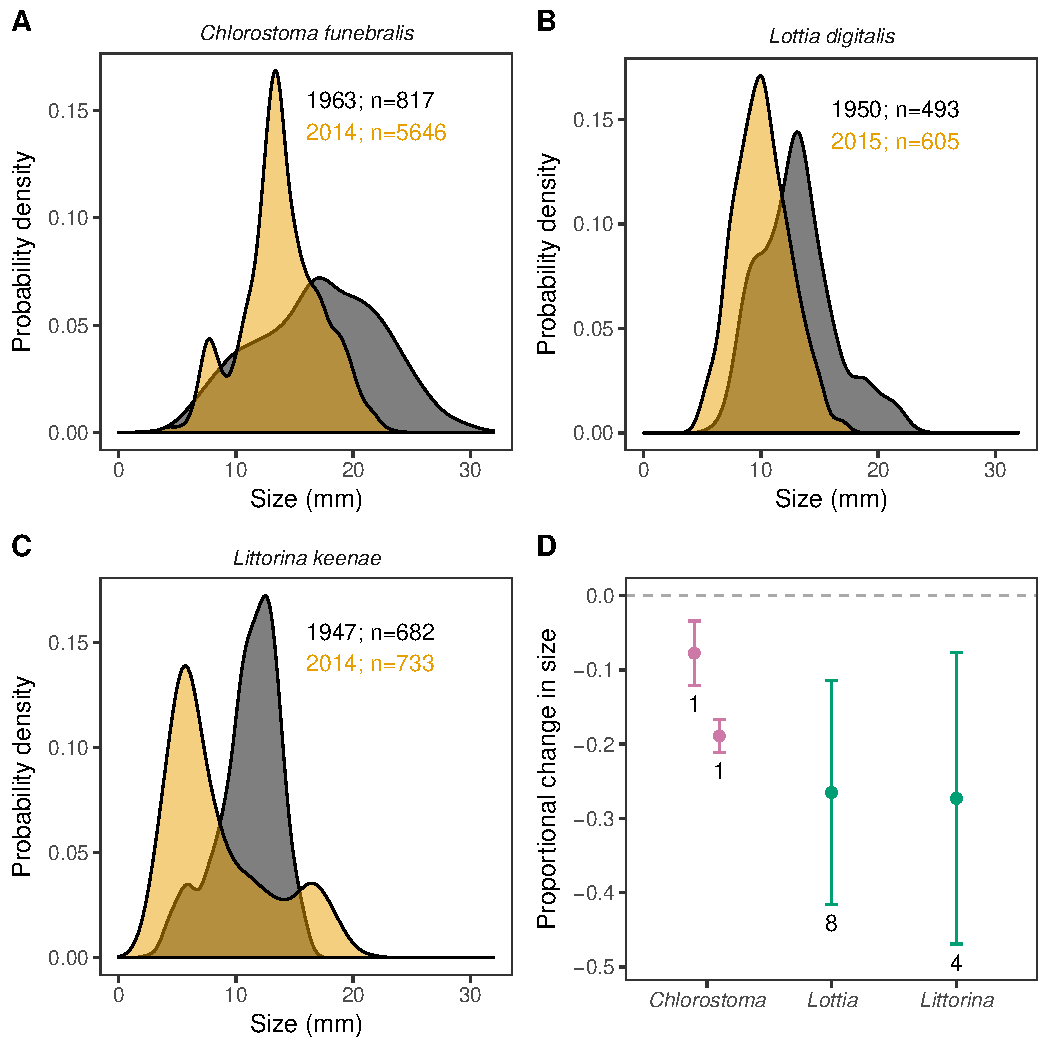
\includegraphics{../../figs_ms/plot_size_frequncy_density_4panel.pdf}
Figure 1. Population-scale reductions in body size were observed for
three intertidal gastropods. Size distributions in the past and present
are presented for \emph{Chlorostoma funebralis} (A), \emph{Lottia
digitalis} (B), and \emph{Littorina keenae} (C), as well as the
proportional reduction in average body size estimated from statistical
models (D). For \emph{Chlorostoma}, \emph{Lottia}, and \emph{Littorina},
snails were measured in 2, 8, and 4 discrete sampling areas,
respectively (see Methods). Therefore, we fit a linear model to each
sampling area for \emph{Chlorostoma} (pink points in (D)), and a
hierarchical linear model across all sampling areas for \emph{Lottia}
and \emph{Littorina} (green points in (D). In (D), the numbers represent
the number of sampling areas used in each model.

\newpage  

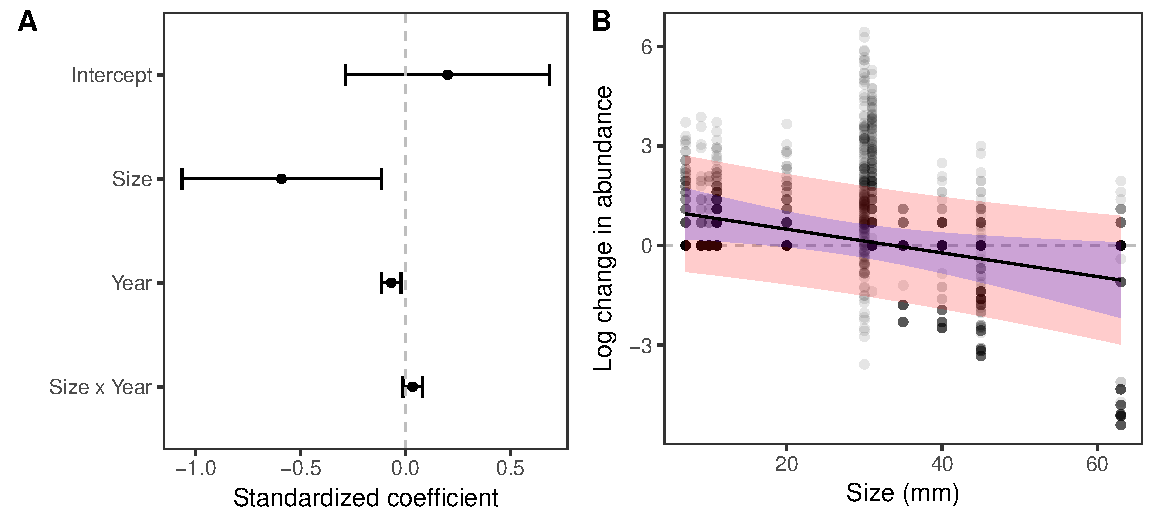
\includegraphics[width=1.00000\textwidth]{../../figs_ms/lrr_herb_size_glmm_2panel.pdf}
Figure 2. Assemblage-scale reductions in body size were observed across
a suite of 11 herbivorous gastropod species between the past (1931) and
present (1993-2015). Relative to 1931, larger snails were less abundant
and smaller snails more abundant. In (A), the fixed effects of size,
year, and their interaction on log change in abundance are presented
with 95\% confidence intervals. In (B), log change in abundance is
plotted against size, with the statistical relationship derived from the
hierarchical linear model. The standard error (in blue) and 95\%
confidence interval (in red) is displayed for the fixed effect of size
(but does not include variation due to the random components of species
or quadrats nested within species).

\newpage 

\subsection{Supplemental Information}\label{supplemental-information}

Table S1. Maximum length (mm) of herbivorous snails observed on the
Hewatt-Sagarin transect. Only 11 species were included in the analysis
(rare species were removed, i.e., those with present in less than 5\% of
samples (n = 228 sampled quadrats)).

\begin{longtable}[]{@{}lrl@{}}
\toprule
Species & Size\_mm & Source\tabularnewline
\midrule
\endhead
Lacuna marmorata & 7 & MAH 1980\tabularnewline
Homalopoma luridum & 9 & MAH 1980\tabularnewline
Tectura paleacea & 10 & MAH 1980\tabularnewline
Lottia asmi & 11 & MAH 1980\tabularnewline
Littorina scutulata/plena & 13 & MAH 1980\tabularnewline
Littorina keenae & 18 & MAH 1980\tabularnewline
Lottia paradigitalis & 20 & Lindberg 1981\tabularnewline
Lottia digitalis & 30 & MAH 1980\tabularnewline
Lottia ochracea & 30 & MAH 1980\tabularnewline
Tegula brunnea & 30 & MAH 1980\tabularnewline
Tegula funebralis & 30 & MAH 1980\tabularnewline
Promartynia pulligo & 30 & MAH 1980\tabularnewline
Acmaea mitra & 35 & MAH 1980\tabularnewline
Lottia pelta & 40 & MAH 1980\tabularnewline
Lottia limatula & 45 & MAH 1980\tabularnewline
Tegula montereyi & 45 & MAH 1980\tabularnewline
Lottia scutum & 63 & MAH 1980\tabularnewline
Haliotis cracherodii & 200 & MAH 1980\tabularnewline
\bottomrule
\end{longtable}

\newpage 

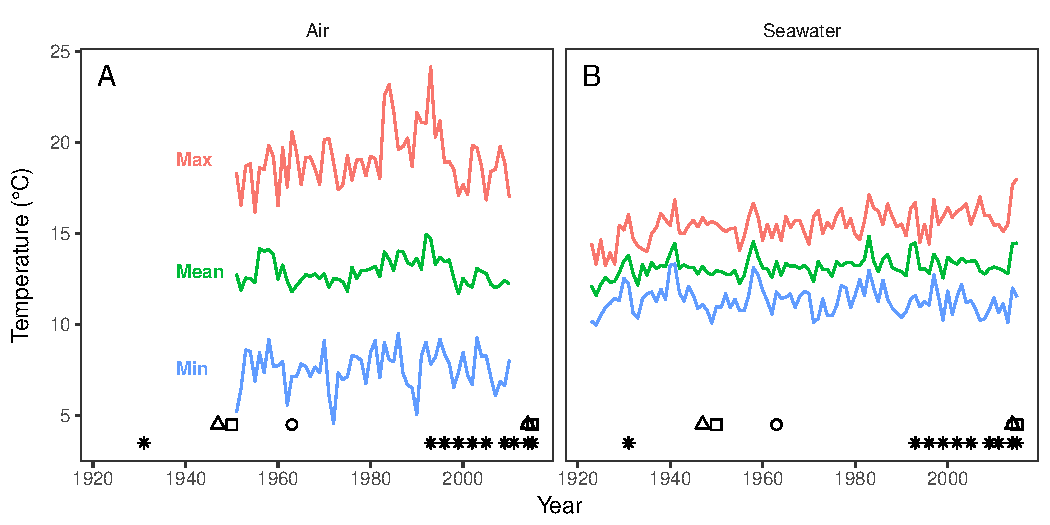
\includegraphics{../../figs_ms/plot_temp_timeseries.pdf} Figure S1. Air
temperatures (A) from a weather station in Monterey (36.6 N, 121.9 E;
2.44km south of the sampling sites; 117m above sea level), and seawater
temperatures (B) from Hopkins Marine Station, Pacific Grove. Asterisks
adjacent to the x-axis represent the temporal samples used in the
`assemblage' test; the open symbols represent the temporal samples used
in the `population' tests of the body size reduction hypothesis (circle,
\emph{Chlorostoma funebralis}; square, \emph{Lottia digitalis},
triangle, \emph{Littorina keenae}).

\textbf{Need to decide on the statistical tests of temperature -
regression, or ANOVA using two time periods. For example, for the
Littorina keenae data, do I use a regression of annual means from
1947-2015, or use an ANOVA to test for a difference in temperature
between 1938-1947 vs 2006-2015?}

\newpage

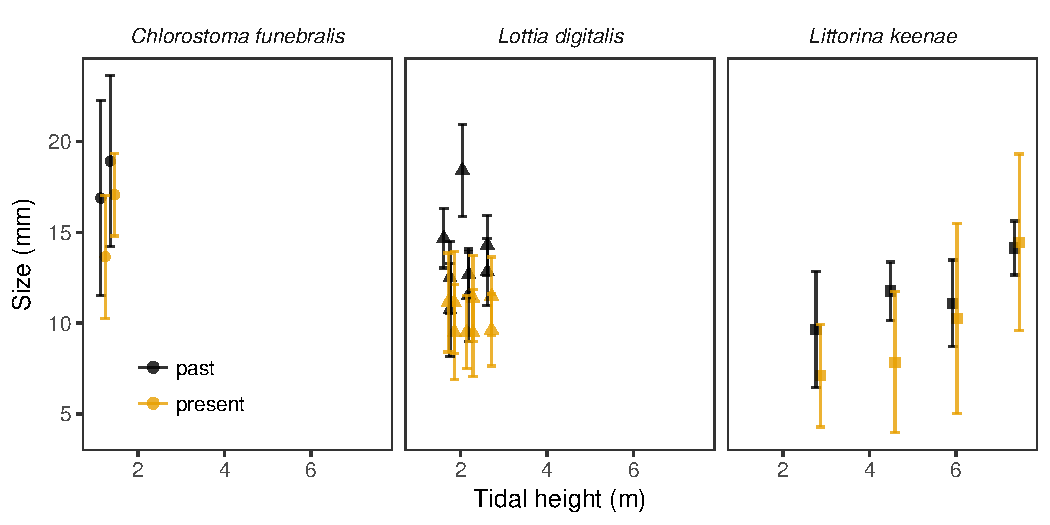
\includegraphics{../../figs_ms/plot_size_era_tide_means.pdf} Figure S2.
Body size (mean +- SD) of three intertidal gastropods plotted against
tidal height. In general, mean body size has declined over six decades.
However, the present size of \emph{L. keenae} (C) has remained similar,
and even larger, in the high intertidal (\textgreater{} 5m above mean
lower low water).

\newpage

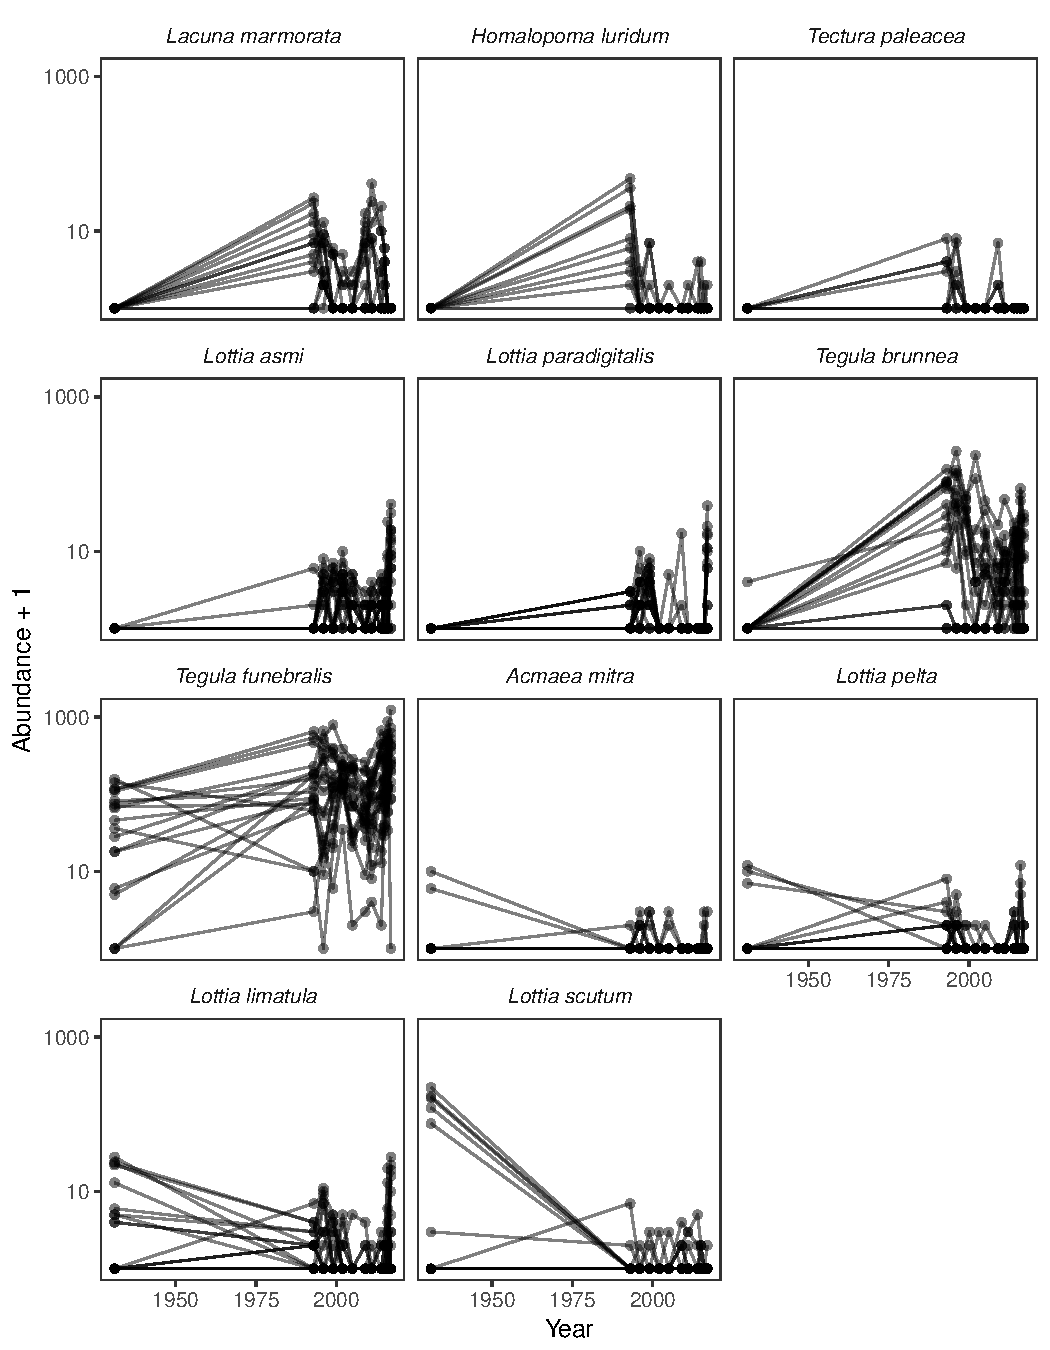
\includegraphics[width=1.00000\textwidth]{../../figs_ms/abund_year_raw_subset_herb.pdf}
Figure S3. Time-series of abundances for herbivorous snails in each of
19 quadrats on the Hewatt-Sagarin transect. These 11 species were used
in the analysis; snails are arranged in order of increasing size.


\end{document}
